\section{Problem 4}
\label{sec:problem4}

The LEO radius follows from the altitude, and the GEO radius from the orbital period (Eq.~1.123 from the course notes):
\begin{equation*}
r_1 = R_E + 300~\text{km} = 6678~\text{km}, \qquad
\tau = 2\pi\sqrt{\frac{r_2^3}{\mu}} \;\Rightarrow\; r_2 = \left(\frac{\mu \tau^2}{4\pi^2}\right)^{1/3}, \qquad
a = \frac{r_1+r_2}{2}
\end{equation*}

\subsection*{(a) and (b) Impulse magnitudes and total $\Delta V$}

The first impulse is tangential (energy change only):
\begin{equation*}
\Delta v_1 = \sqrt{\frac{2\mu}{r_1}-\frac{\mu}{a}} - \sqrt{\frac{\mu}{r_1}}
\end{equation*}
The second impulse circularizes the orbit and rotates the plane by $\theta$ (law of cosines, Eq.~5.53 from the course notes):
\begin{equation*}
\Delta v_2 = \sqrt{(v_2^-)^2 + (v_2^+)^2 - 2v_2^-v_2^+\cos\theta}, \qquad
v_2^- = \sqrt{\frac{2\mu}{r_2}-\frac{\mu}{a}}, \qquad v_2^+ = \sqrt{\frac{\mu}{r_2}}
\end{equation*}
GEO is equatorial ($i_2=0$), so Eq.~5.50 from the course notes gives $\cos\theta = \cos i_1$, i.e.\ $\theta = i_1 = 57^\circ$. The total is
\begin{equation*}
\boxed{\Delta V = \Delta v_1 + \Delta v_2}
\end{equation*}

\subsection*{(c) Time of flight}
Half the period of the transfer orbit:
\begin{equation*}
t_f = \pi\sqrt{\frac{a^3}{\mu}}
\end{equation*}

\subsection*{(d) Mass ratios}
From the rocket equation (Eq.~4.38),
\begin{equation*}
\Delta v = g_0 I_{sp}\ln\left(\frac{m_0}{m_f}\right)
\end{equation*}
so for each impulse
\begin{equation*}
\frac{m_0}{m_f} = \exp\left(\frac{\Delta v_k}{g_0 I_{sp}}\right), \qquad k = 1,2, \qquad I_{sp} = 320~\text{s}
\end{equation*}

\noindent The expressions in parts (a) through (d) are evaluated in \texttt{problem4.py} with $\mu = 398600~\text{km}^3/\text{s}^2$, $R_E = 6378$~km, $\tau = 23.934$~h, $g_0 = 9.80665~\text{m/s}^2$, and $I_{sp} = 320$~s, giving:

\medskip
\programoutput{outputs/problem4.txt}

\subsection*{(e) Hohmann transfer plot}

\begin{figure}[H]
\centering
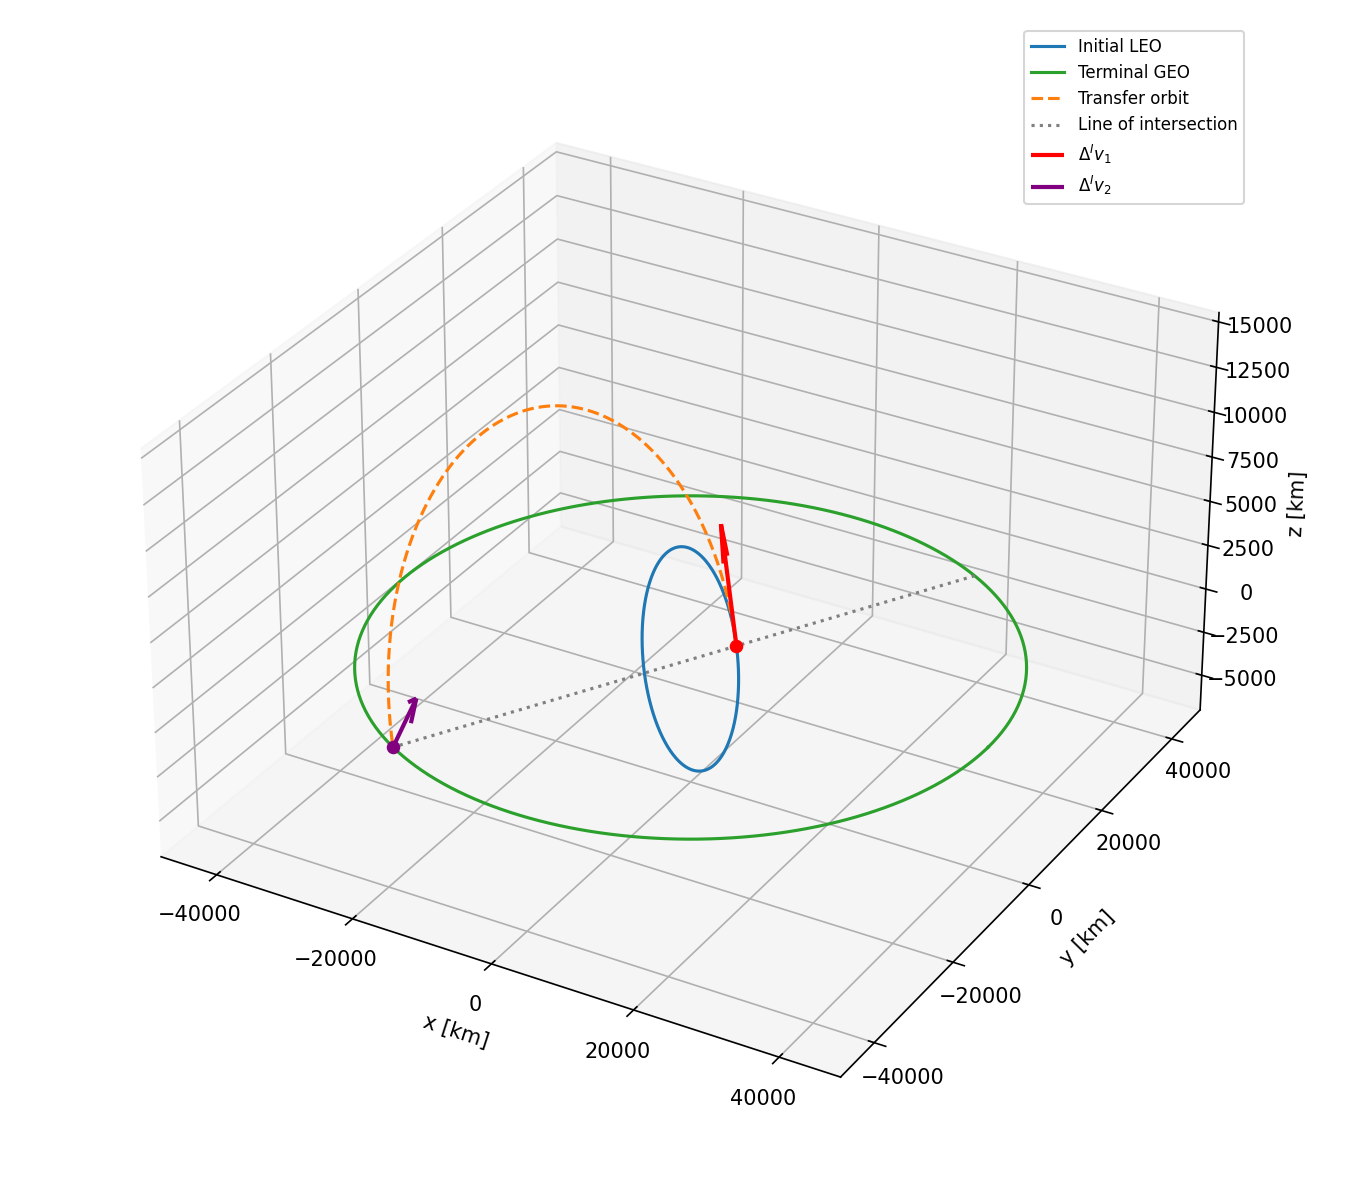
\includegraphics[width=0.8\textwidth]{problem4_transfer.png}
\caption{LEO-to-GEO Hohmann transfer with the plane change at apoapsis.}
\label{fig:p4-transfer}
\end{figure}

\subsection*{(f) Effect of $\Omega$ on the transfer start}

The second impulse must lie on the line of intersection between the initial and terminal orbital planes. Because the terminal orbit is equatorial (GEO), this line of intersection is the line of nodes of the initial orbit. The first impulse is $180^\circ$ away from the second impulse on this same line, so the transfer starts at the opposite node of the initial orbit. Changing $\Omega$ rotates the line of nodes about $\vect{I}_z$, which moves the start point in ECI coordinates, but it is still the node of the initial orbit.
\begin{equation*}
\boxed{\text{No. The transfer always starts at the node of the initial orbit, regardless of }\Omega.}
\end{equation*}

\FloatBarrier
